\chapter{\label{chap:szenarien}Szenarien}
Alle in Kapitel \ref{chap:state} angeführten Technologien haben die Unterstützung der Erstellung von offlinefähigen Anwendungen gemeinsam.
%Sie versprechen, dass die Anwendungen die mit ihnen gebaut werden in der Lage sind mit einer fehlenden Internetverbindung umgehen zu können.\\
% \hyperref[sub:realm]{Realm} verspricht sogar eine automatische Konfliktlösung in Echtzeit.\\
Prinzipiell sollte eine Offline First Anwendung in der Lage sein, mit fehlender Internetverbindung zu funktionieren und mit auftretenden Konflikten so umgehen zu können, dass keine Daten verloren gehen. Sie muss die Fälle behandeln können, die sich aus den folgenden Szenarien ergeben.\\
Im oben beschriebenen Anwendungsfall (Adressbuch) gibt es zwei Parteien die miteinander interagieren: das Adressbuch als Client und den Server. Folgende Situationen können eintreten:
\begin{description}[leftmargin=0.7cm,style=nextline]
% client push
\item[Szenario A0:]
Der Client schickt Daten an den Server, hat den Status \sc{online} und der Server ist erreichbar. Sowohl Anfrage als auch Antwort ist erfolgreich.\\
\item[Szenario A1:]
Der Client schickt Daten an den Server, hat den Status \sc{offline} und der Server ist nicht erreichbar. Die Anfrage schlägt fehl.\\
\item[Szenario A2:]
Der Client schickt Daten an den Server und hat den Status \sc{online}. Die Anfrage wird gestartet und währenddessen bricht die Internetverbindung ab. Die Anfrage `wartet` bis ein Timeout getriggert wird und schlägt dann fehl. Wärend des Wartens ist der Client blockiert.\\
\item[Szenario A3:]
Der Client schickt Daten an den Server und hat den Status \sc{online}. Die Anfrage wird gestartet und währenddessen bricht die Internetverbindung ab. Die Anfrage ist teilweise erfolgreich. Nur ein Teil der gesendeten Daten kommen beim Server an.\\
% client pull / server push
\item[Szenario S0:]
Der Client fordert Daten vom Server an, hat den Status \sc{online} und der Server ist erreichbar. Sowohl Anfrage als auch Antwort ist erfolgreich.\\
\item[Szenario S1:]
Der Client fordert Daten vom Server an, hat den Status \sc{offline} und der Server ist nicht erreichbar. Die Antwort schlägt fehl.\\
\item[Szenario S2:]
Der Client fordert Daten vom Server an und hat den Status \sc{online}. Während der Server antwortet bricht die Internetverbindung ab. Die Antwort `wartet` bis ein Timeout getriggert wird schlägt dann fehl. Wärend des Wartens ist der Client blockiert.\\
\item[Szenario S3:]
Der Client fordert Daten vom Server an und hat den Status \sc{online}. Während der Server antwortet bricht die Internetverbindung ab. Die Antwort ist teilweise erfolgreich. Nur ein Teil der angefragten Daten kommen beim Client an.
\end{description}
In den obigen Szenarien wird nicht beschrieben warum die Internetverbindung abbricht. Dies kann verschiedene Gründe haben. Um nur einige Beispiele zu nennen: Eine langsame Internetverbindung, oder eine Fahrt durch einen Tunnel kann ein Timeout während einer Aktion hervorrufen. Ein auf einer Baustelle gekapptes Kabel oder ein Stromausfall kann zu zeitweise vollständigen Internetverlust (haha) führen.
\begin{figure}[H]
  \centering
  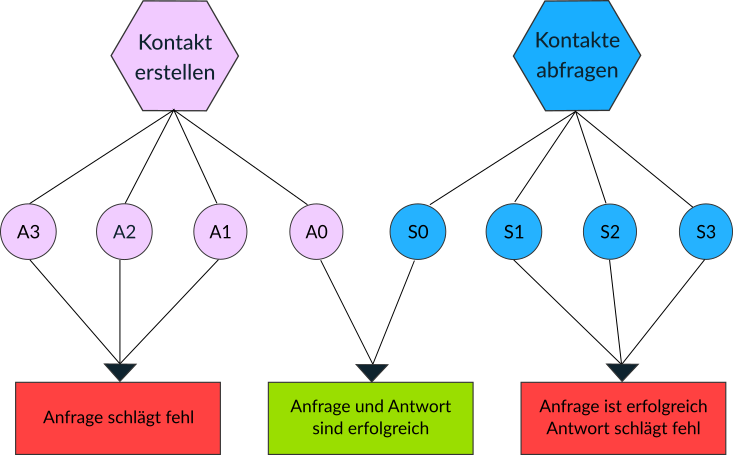
\includegraphics[width=\textwidth]{Szenarien}
  \grayRule
  \caption[Szenarien]{Szenarien und Fälle}
  \label{fig:scenarios}
\end{figure}
%
% ERGEBNIS
%
\subsection*{Ergebnis}
Da die Szenarien \it{A0} und \it{S0}, die Szenarien \it{A1}, \it{A2} und \it{A3} sowie die Szenazien\it{S1}, \it{S2} und \it{S3} zusammengefasst werden können, ergeben sich aus den acht Szenarien die drei nun aufgezählten Fälle.
\begin{itemize}
  \item Fall a: Anfrage und Antwort sind erfolgreich. Es besteht kein Aktionsbedarf \highlight{irrelevant?}
  \item Fall b: Anfrage ist nicht erfolgreich
  \item Fall c: Anfrage ist erfolgreich, Antwort schlägt fehl
\end{itemize}
\highlight{Ergebnis für Fall b und c ist nur aus Entwicklungsperspektive (für die Behandlung) interessant. Das Ergebnis ist identisch: fail}\\
\todo{Anforderungen:}
\it{Die Daten sollten wenigstens so lange auf dem Client gespeichert werden, bis sie vollständig beim Server angekommen sind. Jeder Fehlersfall muss kommuniziert werden. Wenn es konliktbehaftete Daten gibt muss dies mitgeteilt, und angeboten werden die Konflikte zu lösen (Welche Telefonnummer ist die richtige).}